\section{Motivation}
\label{sec:int_motivation}

The success of \ac{GPS} as an outdoor location system and its difficulties to have the same success in the indoor location system's environment sparkled the research for different technologies capable of filling the hole. As such in the last fifteen years many indoor system's have been created which attempted to solve the problem using one or more technologies, each with their strengths and weaknesses. 

With the advancement of smartphones they are now capable of providing many more tools that can be useful for indoor location such as GPS, Wi-Fi, GSM, camera, FM radio, Bluetooth and microphone. Beside these tools, nowadays they even have inertial sensors such as accelerometers, gyroscopes or digital compasses which ,together with ones that were previously mentioned, provide a wide variety of possibilities. Since this field is still in development and there is a big amount of different scenarios in which it has to be applied that consequently brings onto the table different objectives and requirements, every existent solution can be useful for a certain amount of cases due to the nature of each of them. As such there is a huge quantity of existent solutions that have been researched for each technology which then can even branch out according to all the possible optimisations that have to be applied in order to achieved the project's requirements.

This occurrence has led to a need to registrate the state of the indoor location which has been fulfilled by all the existing surveys on the existent technologies \cite{survey1, surveythesis}, which gather up all the existent technologies in the field and analyse them according to their cost, precision, energy efficiency, scalability, privacy, among others criteria. Other surveys analyse technologies on a more specific level by focusing on existent projects to compare their performances \cite{surveywireless}. Another relevant aspect that has been surveyed is the existent techniques utilised \cite{reviewtechniques, survey2, survey3} by analysing the different metrics utilised to calculate a user's position and comparing their strengths and weaknesses according to coverage, line-of-sight and multi-path problems and cost.  

With the situation as is there is big majority of the attention focused on the improving and creating new means to achieve better positioning results, as it is possible to notice from the vast number of existing methods and algorithms available to infer someone's location. Although this part is of great importance, as the success of a location system in the present day is highly dependant on its accuracy levels, another extremely relevant concern for any system is their energetic consumption. With smartphone being the traditional means in any current system, due to its available technologies, it is important to interiorise that it's a personal device with a limited amount of resources, such as battery. 

Another important factor is that an indoor system needs to be scalable, be in function of number of users in the same indoor building or in terms of being capable of working with different deployments/buildings. Systems created with the purpose of being used in multiple different environments need to provide an architecture capable of working seamlessly when transferring between buildings. As such it is required that the one smartphone (mobile agent) capable of working with the system is able to obtaining its own location wherever the system is deployed.  

Since we live in an era dominated by smartphones, their evolution has allowed for developing system which rely on its sensors and processing capacities to present a solution which isn't dependant on specific hardware. With such a dependancy, the first condition that is imposed onto the systems is the compatibility with smartphones, i.e. the required sensors needs to exist on the generic hardware of smartphones. Once this barrier is surpassed, these generic system's are immediately faced with three fundamental decisions which will define the architecture of the system and which can be seen on figure \ref{fig:choices}. The first decision, Technology, defines the technology which is to be used in conjunction with the smartphone and consequently the way that location data is to be collected. There is a wide range of possibilities for this choice, be it BLE beacons, Wi-Fi Access points, LED lamps or just the microphone for sound collection, and each has an impact on the way that the system functions and on its performance. The second question is the location algorithm, which fundamentally depends on the target requirements of the system, if it's required to provide accurate location of a user or if a more descriptive location, such as indicating the room in which the user is located, is enough. There is already a great number of different usable algorithms for each indoor capable technology, as such the choice depends on the way that distance calculation is obtained, be it through time or signal strength, and obviously the technology.The third and last question is about which way will the location be described. When dealing with outdoor location systems, the provided location is always characterized by two values, latitude and longitude, since the existant environment, i.e. the planet Earth, is always the same and as such the coordinates system can be relative to it. In indoor systems, the surrounding environment can be of many shapes and as such different ways of representing the data are necessary. If one thinks about providing indoor location on an office, the precise location isn't as relevant as just knowing the general location, i.e. a building specific description of the location in the form of building, floor and room. On other environments such as supermarkets or even in the previous example, where the objective is to provide more a precise location description, a cartesian coordinate system (x,y) is required.

\begin{figure}[htp]
	\centering
		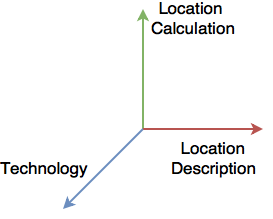
\includegraphics[width=0.5\linewidth]{1.Chapter/vectors.png}
	\caption[Three fundamental choices in Indoor systems]{Three fundamental choices in Indoor systems}
	\label{fig:choices}
\end{figure}

The objective of this work is to present and implement a generic architectural framework whose intent is to provide an architecture where the previously presented requirements are followed. A system implemented on this framework should be capable of bringing the energetic costs of the smartphone to a minimum while allowing itself to be scalable, deployed in multiple sites and reducing the required smartphone space to a minimum.

The previously mentioned generic architecture framework can be visualised in figure \ref{fig:solution}. This architecture makes use of the technologic advancements on mobile phones to use them as the central point of communication of the architecture. This decision may make it seem so that the energetic cost on the smartphone takes a big impact due to the extra effort required for all the communication but it is the opposite as with it being the central piece, i.e. every other element is capable of reaching the smartphone, the data storage and location processing can be externalised onto servers. On this architecture the beacons are responsible for providing the smartphone information about its surroundings, information that is later on passed onto the location server. This server is responsible of computing the user's location and send it back to him. Once the smartphone is aware of its position, he can request the map server and present the result of the whole process visually to the user.

In order to test the idealised architecture, it was necessary to implement a system on it. The chosen technology was the bluetooth low energy, a recent technology that is trying to improve its core in order to be usable on \ac{IoT} and it was capable of providing room-based accuracy without much effort on the algorithm department. The beacon component of the architecture was implement by making use of ble beacon. Each of the used beacons is uniquely identified by its identification and also knows to which location server he belongs to. Whenever a mobile user is nearby an environment where these beacons are present, the mobile user is capable of establishing with them a connection in order to confirm that they do indeed belong to the indoor location system and to access the beacon's data in order to collect information on its owner server.

Once the mobile user has all the data from surrounding devices, i.e. he has data associated to the signals collected from each beacon and the address of their server, he can forward it to the location server. The location server is in possession of a database of all of its associated devices and it is against it that he will compare any data received from mobile users. Upon confirming that the devices belong to it, he can apply its location algorithm to the received data, compute the user's location and send it back to him. 

Upon receiving the user's location, the smartphone is just missing the visual representation of the same location. To do so it sends its location into the map server. The map server in the generic architecture framework represents a server which has a database of all the maps for a certain location server. For this implementation the map server utilised was google maps since its indoor maps feature was available in the testing place. As such, the location of the mobile user is requested to google maps through its API and presented to the user on its smartphone's screen.

%Missing Results


 \begin{figure}[H]
	\centering
		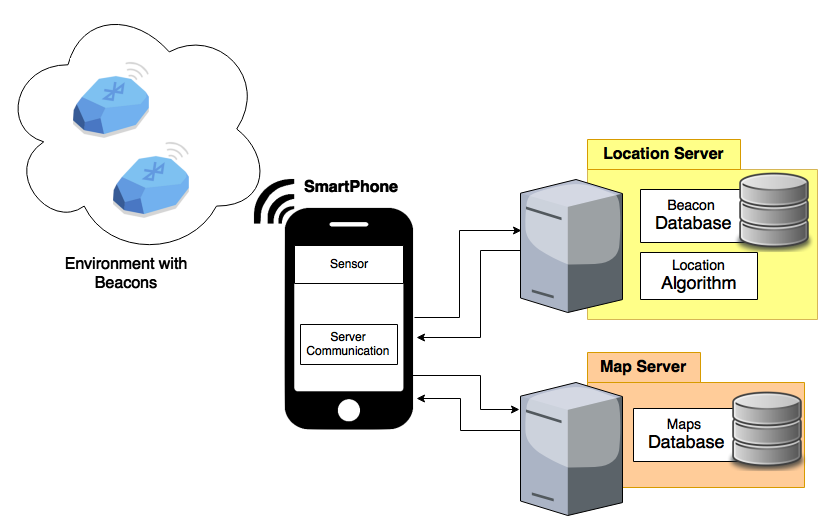
\includegraphics[width=0.5\linewidth]{3.Chapter/generic.png}
	\caption[Generic Architecture Framework]{Generic Architecture Framework }
	\label{fig:solution}
\end{figure}